\documentclass[11pt,a4paper,twocolumn]{article}

% === Core Packages ===
\usepackage[margin=2cm]{geometry}
\usepackage[utf8]{inputenc}
\usepackage[T1]{fontenc}
\usepackage{times}
\usepackage{amsmath,amssymb}
\usepackage{graphicx}
\usepackage{booktabs}
\usepackage{float}
\usepackage{enumitem}
\usepackage{tikz}
\usepackage{pgfplots}
\pgfplotsset{compat=1.18}
\usetikzlibrary{arrows.meta,shapes.geometric,positioning,calc,decorations.markings,fit,backgrounds}

% === Citation (IEEE style) ===
\usepackage[numbers,sort&compress]{natbib}
\bibliographystyle{IEEEtranN}

% === Hyperref ===
\usepackage[hidelinks]{hyperref}
\usepackage{xurl}

% === Settings ===
\setlength{\parindent}{1em}
\setlength{\parskip}{0.3em}

% === Title ===
\title{\textbf{Xarxa de Reputació Descentralitzada:\\Un Marc per a l'Organització Natural de la Societat}}
\author{Pavel Kudrna\\Prague, Czechia\\Esborrany v1 --- Març de 2026}
\date{}

\begin{document}
\maketitle

% ============================================================
% ABSTRACT
% ============================================================
\begin{abstract}
El sentit de la justícia---la convicció que els greuges es reparen i que el mèrit es recompensa---és la força cohesiva més forta de la societat. Quan les institucions centralitzades de govern no poden proporcionar aquest sentit perquè el cost de fer valer un dret supera el valor del dret mateix, la cohesió social s'erosiona. Les estructures institucionals actuals fracassen a resoldre una classe significativa de disputes de manera sistemàticament igual que la planificació central fracassa a assignar recursos: mitjançant l'asimetria d'informació, la manca de bucles de retroalimentació i la desconnexió dels responsables de les decisions respecte de les conseqüències de les seves decisions. Aquest article presenta una Xarxa Social de Reputació (RSN): una capa de comunicació descentralitzada, incorruptible i resistent a la censura, construïda sobre Identificadors Descentralitzats (DID) que permet que participants pseudònims publiquin, verifiquin i consumeixin informació de reputació sobre el comportament al món real. El mecanisme central es fonamenta en tres principis de disseny: (1)~una estructura de costos asimètrica en què llegir dades de reputació és barat però escriure requereix un esforç verificable; (2)~un protocol de selecció de verificadors no determinista basat en el hashing consistent que posa preu a les afirmacions radicals mitjançant costos d'iteració creixents; i (3)~un model d'autoritat de reputació impulsat pel mercat on els verificadors privats arrisquen la seva reputació acumulada sobre l'exactitud de les afirmacions que avalen. L'arquitectura resultant produeix una meritocràcia emergent sense coordinació central i possibilita un camí de migració gradual i reversible des dels sistemes actuals administrats per l'estat.
\end{abstract}

% ============================================================
% 1. INTRODUCTION
% ============================================================
\section{Introducció}

\subsection{El Problema de la Confiança Centralitzada}

El govern modern es basa en una premissa fonamental: que les institucions centralitzades poden mediar la confiança entre desconeguts a gran escala. Els tribunals dirimeixen disputes. Els registres certifiquen la propietat. Els òrgans reguladors fan complir els estàndards. Aquestes institucions van ser dissenyades en una època en què la informació era escassa, la comunicació era lenta i la delegació d'autoritat a un òrgan central era l'únic mecanisme de coordinació factible. El govern centralitzat, però, fracassa per les mateixes raons estructurals que la planificació central: l'asimetria d'informació, la manca de bucles de retroalimentació i la desconnexió dels responsables de les decisions respecte de les conseqüències de les seves decisions.

La premissa fracassa, per exemple, quan el cost de la mediació institucional supera el valor de la disputa. Considereu un llogater que descobreix que l'apartament que ha llogat no té un certificat de seguretat elèctrica legalment obligatori---una condició que suposa un perill immediat per a la vida. El dret legal del llogater a rescindir el contracte és inequívoc. Tanmateix, el cost de fer valer aquest dret a través del sistema judicial supera el valor monetari de la fiança i dels danys deguts, fins i tot incloent-hi una possible compensació legal~\cite{czcourtfees}. La resposta racional és assumir la pèrdua i marxar.

Això no és un cas límit patològic. És l'experiència per defecte per a una classe significativa de disputes en què el dany és real però l'interès monetari cau per sota del llindar en què fer complir la llei institucionalment esdevé econòmicament racional. El resultat és un sistema que estructuralment afavoreix els actors maliciosos: aquells que perjudiquen altres en volums per sota d'aquest llindar poden actuar amb impunitat, perquè el cost de cercar justícia recau sobre la part perjudicada.

L'exemple anterior prové de l'entorn jurídic de l'autor---el sistema de dret civil txec. En altres tradicions jurídiques---el dret comú basat en precedents, el dret consuetudinari, els sistemes mixtos---la justícia fracassa de maneres diferents i en graus diferents, segons les especificitats culturals i procedimentals de la jurisdicció. Els lectors probablement reconeixeran exemples equivalents del seu propi context. El que és estructuralment universal és el patró: les disputes el valor de les quals cau per sota del llindar de compliment econòmicament racional acaben amb la pèrdua assumida per la part perjudicada. La RSN no promet una justícia perfecta---només redueix l'avantatge estructural que gaudeixen els actors maliciosos quan el compliment institucional no és econòmic.

\subsection{Per què les Solucions Existents es Queden Curtes}

\textbf{Els marcs d'Identitat Descentralitzada (DID)}~\cite{did2022} proporcionen mecanismes criptogràfics per a la gestió d'identitat autosobirana però se centren principalment en la verificació d'identitat sense abordar la qüestió més àmplia de la reputació comportamental.

\textbf{Els Soulbound Tokens (SBT)}~\cite{weyl2022} recullen la idea que la reputació és intransferible però depenen d'infraestructura de blockchain amb restriccions d'escalabilitat i no aborden els incentius econòmics que regeixen l'entrada d'informació. Conceptes relacionats com els merit tokens (p.\ ex., Liberland) comparteixen una filosofia semblant però romanen lligats a marcs jurisdiccionals específics.

\textbf{Les Organitzacions Autònomes Descentralitzades (DAO)}~\cite{buterin2014} implementen la governança mitjançant contractes intel·ligents però reprodueixen dinàmiques plutocràtiques on la influència és proporcional al capital. La votació quadràtica~\cite{buterin2019} ho mitiga parcialment però limita l'adopció pràctica. Les DAO també s'enfronten al \emph{problema de l'oracle} fonamental: els contractes intel·ligents no poden verificar de manera fiable els estats del món real sense una font externa de confiança, i aquest problema no té solució general dins l'arquitectura de blockchain.

Cap sistema existent combina descentralització, resistència a la censura, pseudonímia, cost d'entrada verificable i consens emergent.

\subsection{Contribucions}

Aquest article fa les contribucions següents:
\begin{enumerate}[nosep]
\item Definició de la \textbf{Xarxa Social de Reputació (RSN)}, un protocol descentralitzat que estén el marc DID per donar suport a l'intercanvi bilateral de reputació.
\item Un \textbf{protocol de selecció de verificadors no determinista} basat en el hashing consistent~\cite{karger1997}.
\item El \textbf{Principi del Radicalisme Costós}, que posa preu a les afirmacions segons la seva distància respecte del consens de la xarxa mitjançant tres canals de cost acumulatius.
\item Un \textbf{model d'Autoritat de Reputació} amb incentius asimètrics on l'aval fals costa catastròficament més que les comissions legítimes.
\item Un \textbf{camí de migració gradual} a través d'una infraestructura fiscal paral·lela.
\end{enumerate}

% ============================================================
% 2. DESIGN PRINCIPLES
% ============================================================
\section{Principis de Disseny}

L'arquitectura de la RSN està restringida per cinc principis de disseny innegociables.

\textbf{Continuïtat i Evolució.} El sistema coexisteix amb les institucions existents durant un període de transició de durada indefinida. La transició ha de ser reversible en cada etapa.

\textbf{Voluntarietat i Responsabilitat.} La participació és voluntària, però la voluntarietat va lligada a la responsabilitat: un participant que assumeix el control sobre una funció institucional assumeix simultàniament les obligacions que hi corresponen.

\textbf{Diversitat i Neutralitat Cultural.} El consens emergeix de les interaccions bilaterals, no de regles predefinides imposades pels dissenyadors del sistema.

\textbf{Resiliència i Resistència a la Censura.} El cost de censurar la xarxa ha de superar el cost de tolerar-la. Només un totalitarisme complet---a un cost polític i econòmic ruïnós---pot suprimir el sistema.

\textbf{Consens i Compliment.} El sistema incorpora les tendències humanes a la mesquinesa, el ressentiment i la satisfacció retributiva com a característiques portants. La mala conducta no es prohibeix; se li posa preu.

% ============================================================
% 3. SYSTEM OVERVIEW
% ============================================================
\section{Visió General del Sistema}

\subsection{Xarxa Social de Reputació}

La RSN és una capa de comunicació descentralitzada i entre iguals en què els participants intercanvien informació verificable sobre el comportament al món real. Les seves propietats definitòries són: infraestructura descentralitzada i incensurable; participació pseudònima mitjançant DID; estructura de costos asimètrica (llegir és barat, escriure és car); verificabilitat criptogràfica; i \textbf{suport a estàndards}---formats llegibles per màquina per a la informació propagada a través de la xarxa, per als serveis oferts per les autoritats (composició d'afirmacions, aval, servei de testimoni), i per al format de política incloent-hi regles per avaluar la reputació de la contrapart i valorar el risc de discrepància de política (entre el comportament declarat i el real).

\subsection{Components Arquitectònics}

La RSN consta de quatre components principals (Fig.~\ref{fig:architecture}):
\begin{enumerate}[nosep]
\item \textbf{Capa DID.} Identitats de participants amb regles declarades, metadades de reputació i encaminament de xarxa.
\item \textbf{Protocol d'Afirmacions.} Format estructurat per publicar asseveracions sobre esdeveniments del món real.
\item \textbf{Xarxa de Verificació.} Protocol descentralitzat per assignar verificadors mitjançant el hashing consistent.
\item \textbf{Capa d'Agregació de Reputació.} Serveis que produeixen resums de reputació llegibles per humans.
\end{enumerate}

\begin{figure}[ht]
\centering
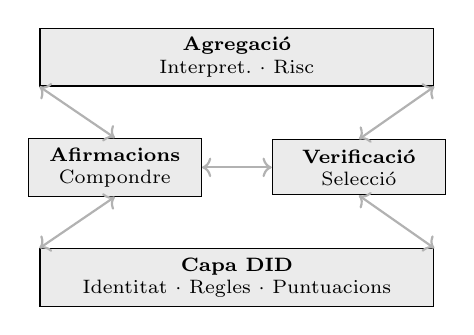
\begin{tikzpicture}[
    layer/.style={draw, minimum height=0.7cm, align=center, font=\scriptsize, fill=black!8},
    arr/.style={<->, thick, gray!60}
]
\node[layer, minimum width=5cm] (agg) at (0,2.8) {\textbf{Agregació}\\Interpret.\ $\cdot$ Risc};
\node[layer, minimum width=2.2cm] (claim) at (-1.55,1.4) {\textbf{Afirmacions}\\Compondre};
\node[layer, minimum width=2.2cm] (verif) at (1.55,1.4) {\textbf{Verificació}\\Selecció};
\node[layer, minimum width=5cm] (did) at (0,0) {\textbf{Capa DID}\\Identitat $\cdot$ Regles $\cdot$ Puntuacions};

\draw[arr] (agg.south west) -- (claim.north);
\draw[arr] (agg.south east) -- (verif.north);
\draw[arr] (claim.east) -- (verif.west);
\draw[arr] (claim.south) -- (did.north west);
\draw[arr] (verif.south) -- (did.north east);
\end{tikzpicture}
\caption{Arquitectura de quatre capes de la RSN.}
\label{fig:architecture}
\end{figure}

\subsection{Rols dels Participants}

Una transacció de verificació implica fins a sis rols DID diferents (Fig.~\ref{fig:roles}): \textbf{Emissor} ($DID_I$, crea i tramet l'afirmació), \textbf{Subjecte} ($DID_S$, el DID de qui tracta l'afirmació---pot coincidir amb l'Emissor), \textbf{Autoritat} ($DID_A$, avala l'afirmació a canvi d'una comissió; també pot oferir serveis de testimoni---\emph{opcional}), \textbf{Testimoni} ($DID_{W_{1..n}}$, supervisor d'incògnit de l'honestedat del verificador mitjançant codis de repte---\emph{opcional}), \textbf{Verificador} ($DID_V$, seleccionat algorísmicament per publicar l'afirmació), i la \textbf{RSN} (la xarxa on es publiquen les afirmacions verificades). Qualsevol rol es pot delegar a un altre DID (Secció~7.4). Una Autoritat sovint agrupa l'aval amb els serveis de testimoni, però les dues funcions són lògicament independents.

\begin{figure}[ht]
\centering
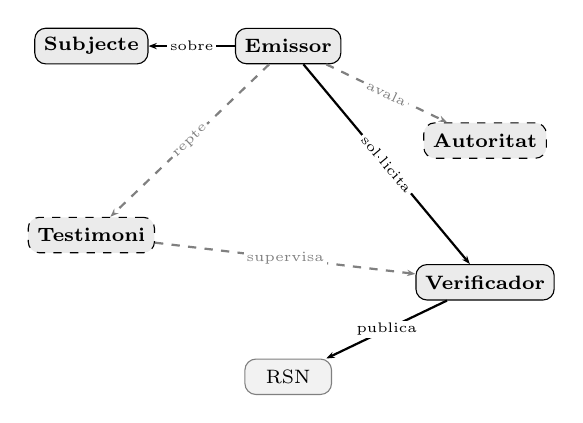
\begin{tikzpicture}[
    role/.style={draw, rounded corners, minimum width=1.1cm, minimum height=0.45cm, align=center, font=\scriptsize, fill=black!8},
    opt/.style={draw, rounded corners, minimum width=1.1cm, minimum height=0.45cm, align=center, font=\scriptsize, fill=black!8, dashed},
    arr/.style={-{Stealth[length=3pt]}, thick},
    oarr/.style={-{Stealth[length=3pt]}, thick, dashed, gray},
    lbl/.style={font=\tiny, fill=white, inner sep=1pt}
]
\node[role] (I) at (0,2.4) {\textbf{Emissor}};
\node[role] (S) at (-2.5,2.4) {\textbf{Subjecte}};
\node[opt] (A) at (2.5,1.2) {\textbf{Autoritat}};
\node[opt] (W) at (-2.5,0) {\textbf{Testimoni}};
\node[role] (V) at (2.5,-0.6) {\textbf{Verificador}};
\node[role, fill=black!5, draw=gray] (N) at (0,-1.8) {RSN};

\draw[arr] (I) -- node[lbl] {sobre} (S);
\draw[oarr] (I) -- node[lbl,sloped] {avala} (A);
\draw[oarr] (I) -- node[lbl,sloped] {repte} (W);
\draw[arr] (I) -- node[lbl,sloped] {sol·licita} (V);
\draw[oarr] (W) -- node[lbl] {supervisa} (V);
\draw[arr] (V) -- node[lbl] {publica} (N);
\end{tikzpicture}
\caption{Rols DID en una transacció de verificació. Discontinu = opcional (Autoritat, Testimoni).}
\label{fig:roles}
\end{figure}

\subsection{Incorruptibilitat: Quatre Forces}

La incorruptibilitat de la RSN no sorgeix d'un únic mecanisme sinó de quatre forces concurrents. Cap no és suficient per si sola; només la seva combinació fa que un intent de corrupció sigui econòmicament irracional.

\textbf{Objectiu impredictible.} El verificador de cada afirmació se selecciona de manera no determinista mitjançant el hashing consistent (Secció~5.3). Un atacant no pot preseleccionar un verificador concret per subornar-lo, perquè la identitat del verificador és funció del contingut de l'afirmació i de les iteracions anteriors, no de l'elecció de l'emissor.

\textbf{Palanquejament reputacional---lent a l'alça, ràpid a la baixa.} La reputació només es pot guanyar de manera incremental, mitjançant un comportament consistent i sostingut. Pot, però, perdre's catastròficament en un únic aval fraudulent (Secció~6.2). Aquesta asimetria significa que anys de reputació acumulada es poden destruir amb un sol aval deshonest; l'estratègia òptima continua sent rebutjar les afirmacions sospitoses.

\textbf{Promesa pública.} Cada Titular de DID declara públicament la seva política---un conjunt de regles llegibles per màquina que es compromet a seguir. La divergència entre la declaració i el comportament real és detectable i se li posa preu com una infracció reputacional més greu que la violació subjacent (Secció~7.3). Per tant, la hipocresia és més costosa que la deshonestedat directa.

\textbf{Asimetria del cost d'atac a la malla.} El cost de censurar o desestabilitzar la xarxa creix de manera no lineal amb la mida i la densitat de la xarxa, mentre que el cost de tolerar-la roman constant. Perquè la censura fos rendible, un actor centralitzat hauria d'aplicar-la a tota la xarxa---requerint mesures desproporcionades respecte de qualsevol benefici concebible (Secció~10).

% ============================================================
% 4. DECENTRALIZED IDENTITY MODEL
% ============================================================
\section{Model d'Identitat Descentralitzada}

\subsection{DID amb Propietats Especials}

La RSN estén l'especificació W3C DID Core~\cite{did2022} amb: \textbf{Regles Declarades} (compromisos comportamentals llegibles per màquina), \textbf{Metadades de Reputació} (puntuació comportamental agregada) i \textbf{Encaminament de Xarxa} (passarel·la onion mutable separada de la posició estable a l'anell).

\subsection{Cicle de Vida de l'Afirmació}

Una Afirmació avança a través de sis etapes (Fig.~\ref{fig:lifecycle}): composició, aval d'autoritat opcional, selecció de verificador mitjançant el hashing consistent, decisió de verificació (acceptar o rebutjar amb iteració), publicació i actualització de reputació per a totes les parts.

\begin{figure}[ht]
\centering
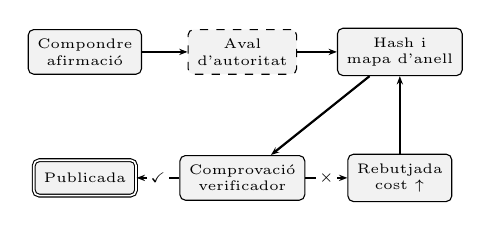
\begin{tikzpicture}[
    stp/.style={draw, rounded corners=2pt, minimum width=1.3cm, minimum height=0.45cm, align=center, font=\tiny, fill=black!5},
    arr/.style={-{Stealth[length=3pt]}, thick},
    lbl/.style={font=\tiny, fill=white, inner sep=1pt}
]
\node[stp] (comp) at (0,0) {Compondre\\afirmació};
\node[stp, dashed] (auth) at (2.0,0) {Aval\\d'autoritat};
\node[stp] (hash) at (4.0,0) {Hash i\\mapa d'anell};
\node[stp] (ver) at (2.0,-1.6) {Comprovació\\verificador};
\node[stp, double] (pub) at (0,-1.6) {Publicada};
\node[stp] (rej) at (4.0,-1.6) {Rebutjada\\cost $\uparrow$};

\draw[arr] (comp) -- (auth);
\draw[arr] (auth) -- (hash);
\draw[arr] (hash) -- (ver);
\draw[arr] (ver) -- node[lbl] {\checkmark} (pub);
\draw[arr] (ver) -- node[lbl] {$\times$} (rej);
\draw[arr] (rej) -- ++(0,0.8) -| (hash);
\end{tikzpicture}
\caption{Cicle de vida de l'afirmació amb bucle d'iteració.}
\label{fig:lifecycle}
\end{figure}

\subsection{Relació amb W3C DID Core}

El model d'identitat de la RSN és un superconjunt propi de l'especificació W3C DID Core~\cite{did2022}. Tots els DID de la RSN són DID vàlids del W3C. Les extensions específiques de la RSN es codifiquen com a propietats del document DID definides en una especificació de mètode DID dedicada, compatible amb infraestructura existent com ION~\cite{buchner2021} i Ceramic~\cite{ceramic2023}.

% ============================================================
% 5. VERIFICATION AND PROPAGATION
% ============================================================
\section{Verificació i Propagació de la Informació}

\subsection{Cost d'Entrada de la Informació}

El principi econòmic central de la RSN és l'asimetria entre llegir i escriure. Llegir dades de reputació s'acosta a un cost marginal zero per als participants que formen part de la xarxa DID i tenen accés proporcional a la seva reputació---els nouvinguts han de guanyar-se gradualment un accés més ampli (vegeu antiparasitisme). Escriure---entès com la materialització duradora de la reputació a la xarxa, no com un acte tècnic puntual---requereix una inversió acumulada verificable en tres dimensions: \textbf{temps} (anys de vida dedicats a un comportament consistent, compromisos complerts i relacions cultivades), \textbf{energia} (esforç invertit en el tracte honest, la cura de les associacions i la fiabilitat a llarg termini), i \textbf{diners} (inversió en el propi nom---desenvolupament professional, la qualitat de la pròpia feina, la restitució dels danys causats). La reputació no es pot comprar a l'instant---és el resultat d'una acumulació de tota una vida que el sistema es limita a fer visible i transferible entre contextos. Els costos tècnics puntuals del protocol (signatures criptogràfiques, comissions de verificador) són negligibles en comparació amb aquesta inversió subjacent.

\subsection{Graf Social i Profunditat de Contactes}

La RSN és fonamentalment una xarxa social: cada DID afegeix contactes (altres DID) que permeten la connexió. Aquests contactes tenen els seus propis contactes, i així successivament. La cerca algorísmica de verificadors opera dins d'una profunditat configurable $h$ de contactes enllaçats (p.\ ex., $h=3$: els contactes directes propis, els seus contactes, i els contactes dels contactes). Aquesta arquitectura no requereix una única blockchain global---afavoreix naturalment l'aparició de comunitats/clústers amb solapaments cap a altres comunitats. Cada participant DID ha de tenir una \textbf{política} publicada---un conjunt de regles llegibles per màquina que regeix com s'avaluen les sol·licituds entrants. Les violacions de política es registren a la xarxa com a artefactes negatius.

\subsection{Selecció Algorísmica de Verificadors}

El protocol de verificació empra el hashing consistent~\cite{karger1997} (Fig.~\ref{fig:verifier}). La verificació és un servei de pagament: els verificadors operen a canvi d'una comissió, creant un mercat on la competència impulsa el preu, la rapidesa i la fiabilitat.

\textbf{Pas 1.} El document de l'afirmació es concatena amb el resultat del hash de la iteració anterior (o $\varnothing$ en la primera iteració) i s'aplica el hash:
\begin{equation}
\text{pos} = f_h(\text{claim} \| \text{prev\_hash})
\label{eq:hash}
\end{equation}

L'algorisme ha d'incloure el \emph{camí complet} de totes les sol·licituds i respostes anteriors---no simplement un hash de la iteració anterior. La resposta completa de cada verificador (acceptació, rebuig, preu cotitzat, motiu) s'annexa al document creixent, verificable mitjançant signatures criptogràfiques a cada pas.

\textbf{Pas 2.} El hash es mapeja a $N$ posicions a l'anell de hash consistent, distribuïdes uniformement (p.\ ex., per a $N=4$: $+0^{\circ}, +90^{\circ}, +180^{\circ}, +270^{\circ}$). Des de cada posició, una cerca en sentit horari selecciona el DID més proper com a candidat a verificador (Fig.~\ref{fig:multipoint}). $N$ és un paràmetre variable que pot dependre del percentatge de DID actualment actius, de l'hora del dia, o de la capacitat de resposta històrica de la xarxa.

\textbf{Pas 3.} El Verificador accepta (publica, arriscant reputació) o rebutja (tornant al Pas~1 amb el hash del rebuig). Quan un node no respon tot i declarar estat en línia, la sol·licitud següent ha d'incloure totes les respostes de tots els $N$ candidats a verificador anteriors.

\textbf{Antiparasitisme.} Els DID objectiu poden fixar comissions o restriccions d'accés per a consultes de DID nous amb poca reputació. Aquest mecanisme graduat (no binari) obliga els nouvinguts a construir reputació mitjançant una activitat genuïna abans de consumir lliurement les dades d'altres.

\begin{figure}[ht]
\centering
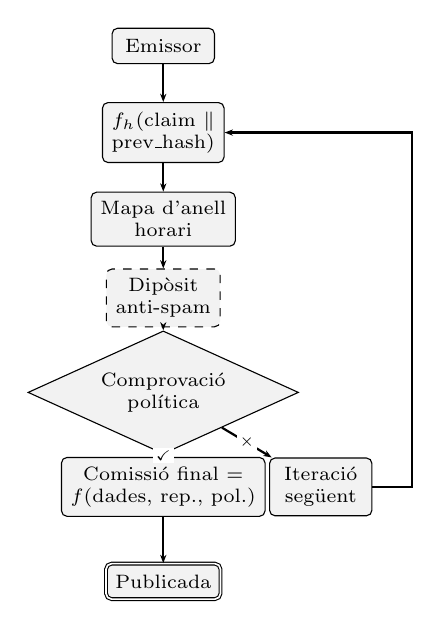
\begin{tikzpicture}[
    box/.style={draw, rounded corners=2pt, minimum width=1.3cm, minimum height=0.45cm, align=center, font=\scriptsize, fill=black!5},
    dec/.style={draw, diamond, aspect=2.2, minimum width=0.9cm, align=center, font=\scriptsize, fill=black!5},
    arr/.style={-{Stealth[length=3pt]}, thick},
    lbl/.style={font=\tiny, fill=white, inner sep=1pt}
]
\node[box] (iss) at (0,0) {Emissor};
\node[box] (hash) at (0,-1.1) {$f_h$(claim $\|$\\prev\_hash)};
\node[box] (ring) at (0,-2.2) {Mapa d'anell\\horari};
\node[box, dashed] (spam) at (0,-3.2) {Dipòsit\\anti-spam};
\node[dec] (check) at (0,-4.4) {Comprovació\\política};
\node[box] (rej) at (2,-5.6) {Iteració\\següent};
\node[box] (fee) at (0,-5.6) {Comissió final =\\$f$(dades, rep., pol.)};
\node[box, double] (pub) at (0,-6.8) {Publicada};

\draw[arr] (iss) -- (hash);
\draw[arr] (hash) -- (ring);
\draw[arr] (ring) -- (spam);
\draw[arr] (spam) -- (check);
\draw[arr] (check) -- node[lbl] {$\times$} (rej);
\draw[arr] (check) -- node[lbl] {\checkmark} (fee);
\draw[arr] (fee) -- (pub);
\draw[arr] (rej.east) -- ++(0.5,0) |- (hash.east);
\end{tikzpicture}
\caption{Protocol de selecció de verificador. El dipòsit anti-spam és opcional i pot ser reemborsable. La comissió final es paga només en cas d'acceptació.}
\label{fig:verifier}
\end{figure}

Cada rebuig annexa la resposta completa del verificador (incloent-hi motius i condicions) al document de l'afirmació, ampliant-ne el contingut. A partir del document ampliat, es computa un nou hash de manera no determinista, mapejant a una posició d'anell diferent i seleccionant un verificador diferent. La documentació del camí complet és obligatòria---l'emissor no pot predir ni influir en el verificador següent. Si un verificador ignora una sol·licitud tot i tenir una política declarada compatible, els testimonis (si n'hi ha) ho registren, i l'emissor pot adjuntar les proves dels testimonis en la publicació final.

\begin{figure}[ht]
\centering
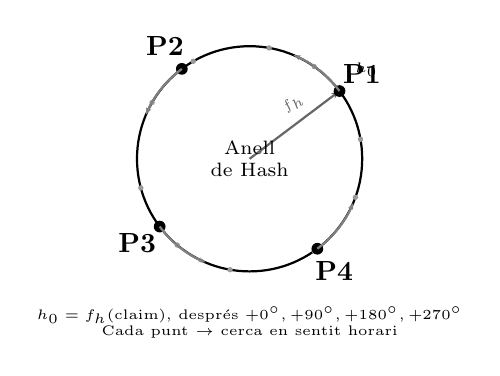
\begin{tikzpicture}[scale=0.65]
% Ring
\draw[thick] (0,0) circle (2.2cm);
% DID nodes on ring
\foreach \a in {10,55,80,120,150,195,230,260,305,340} {
  \fill[black!40] (\a:2.2) circle (1.5pt);
}
% Hash offset arrow pointing to initial position
\draw[-{Stealth[length=3pt]}, thick, black!60] (0,0) -- node[font=\tiny,above,sloped,pos=0.6] {$f_h$} (37:2.2);
\fill[black] (37:2.2) circle (2pt);
\node[font=\tiny,anchor=south west] at (37:2.35) {$h_0$};
% N=4 points offset from h0 by +0, +90, +180, +270
\foreach \offset/\l in {0/P1,90/P2,180/P3,270/P4} {
  \pgfmathsetmacro{\ang}{37+\offset}
  \node[fill=black, circle, inner sep=1.5pt] (p\offset) at (\ang:2.2) {};
  \node[font=\tiny,font=\bfseries] at (\ang:2.75) {\l};
  % clockwise search arc
  \draw[-{Stealth[length=2.5pt]}, thick, gray] (\ang:2.2) arc (\ang:\ang+30:2.2);
}
\node[font=\scriptsize, align=center] at (0,0) {Anell\\de Hash};
\node[font=\tiny, align=center] at (0,-3.2) {$h_0 = f_h(\text{claim})$, després $+0^{\circ},+90^{\circ},+180^{\circ},+270^{\circ}$\\Cada punt $\rightarrow$ cerca en sentit horari};
\end{tikzpicture}
\caption{Selecció multipunt ($N{=}4$). El hash $h_0$ fixa el desplaçament; 4 punts distribuïts uniformement des de $h_0$.}
\label{fig:multipoint}
\end{figure}

\subsection{Protocol de Testimoni}

El rol de \textbf{Testimoni} proporciona responsabilitat d'incògnit per a l'honestedat del verificador mitjançant un protocol criptogràfic de codis de repte:

\textbf{Pas W1.} El sol·licitant signa la sol·licitud de verificació i l'envia a $N_w$ testimonis---contactes de la xarxa social del sol·licitant, o proveïdors especialitzats de serveis de testimoni que operen a canvi d'una comissió.

\textbf{Pas W2.} Cada testimoni $w_i$ signa tota la sol·licitud signada, reté la signatura original $\sigma_i$, i computa un codi de repte $c_i = h(\sigma_i)$. El codi de repte s'annexa a la sol·licitud.

\textbf{Pas W3.} La sol·licitud, ara portant $N_w$ codis de repte, s'envia al verificador. El verificador observa els codis però \emph{no pot determinar} qui són els testimonis ni si els codis corresponen a signatures reals.

\textbf{Pas W4 (verificador honest).} Si el verificador respon d'acord amb la seva política declarada, els codis de repte romanen opacs. Els testimonis no es revelen mai. No es publica cap dada addicional.

\textbf{Pas W5 (violació de política).} Si el verificador viola la seva política (ignora la sol·licitud, respon de manera inconsistent), el sol·licitant conserva les signatures originals dels testimonis $\sigma_i$. Aquestes es poden publicar com a dades acompanyants: qualsevol pot verificar $c_i = h(\sigma_i)$, provant que el testimoni hi era present. El sol·licitant pot publicar de manera independent---el verificador ja havia signat els codis de repte en la seva resposta.

\textbf{La propietat del catxa.} El sol·licitant pot substituir alguns o tots els codis de repte per valors aleatoris. El verificador no pot distingir els codis genuïns (respatllats per autoritats d'alta reputació) del soroll. Aquesta \emph{incertesa} és el mecanisme de compliment: cada sol·licitud comporta el risc que una autoritat respectada estigui vigilant d'incògnit. El cost de mantenir aquesta pressió és pràcticament zero (generar nombres aleatoris), mentre que el cost potencial de la deshonestedat per al verificador és catastròfic. El comportament honest s'incentiva fins i tot en absència de testimonis reals.

\textbf{L'Autoritat com a testimoni.} Una Autoritat que avala una afirmació pot agrupar-hi serveis de testimoni: ``Avalo la teva afirmació i actuo com a testimoni d'incògnit durant la verificació.'' Aquest és un model de negoci natural---l'Autoritat ja disposa del context. Tanmateix, els dos rols són lògicament independents.

\subsection{Principi del Radicalisme Costós}

Tres canals de cost es componen simultàniament (Fig.~\ref{fig:radicalism}):

\textbf{Canal 1: Cost d'Iteració.} Cada rebuig força una nova iteració que consumeix temps i recursos. Creixement lineal.

\textbf{Canal 2: Inflament del Document.} Cada iteració afegeix la resposta completa del verificador al document de l'afirmació. El creixement és lineal, però amb un desplaçament base: la càrrega inicial (contingut de l'afirmació, aval d'autoritat, signatures criptogràfiques) ja té una mida no trivial $B_0$. Mida total després de $k$ iteracions: $S(k) = B_0 + k \cdot \Delta$, on $\Delta$ és la mida mitjana de la resposta.

\textbf{Canal 3: Prima de Risc del Verificador.} El risc és subjectiu. El verificador avalua si les polítiques declarades del DID sol·licitant entren en conflicte amb els interessos comercials, socials o polítics del propi verificador. La prima pot escalar exponencialment amb la distància percebuda respecte de l'``ideal'' del verificador: $P(d) = \alpha \cdot e^{\beta d}$, on $d$ és la mètrica de distància subjectiva del verificador. Més enllà d'un límit personal infranquejable, el verificador pot negar-s'hi del tot.

\begin{figure}[ht]
\centering
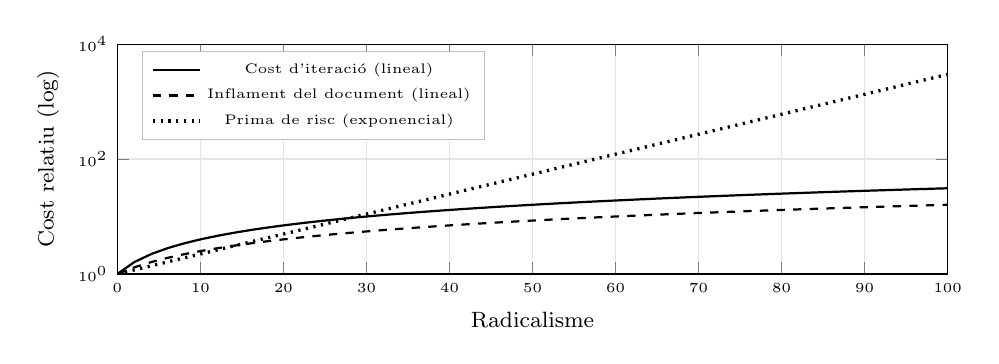
\begin{tikzpicture}
\begin{axis}[
    width=\columnwidth,
    height=4.5cm,
    xlabel={\footnotesize Radicalisme},
    ylabel={\footnotesize Cost relatiu (log)},
    ymode=log,
    xmin=0, xmax=100,
    ymin=1, ymax=10000,
    grid=major,
    grid style={gray!20},
    legend style={at={(0.03,0.97)},anchor=north west,font=\tiny,draw=gray!50},
    tick label style={font=\tiny},
    label style={font=\footnotesize},
]
\addplot[black, thick, domain=0:100, samples=50] {1 + 0.3*x};
\addlegendentry{Cost d'iteració (lineal)}
\addplot[black, thick, dashed, domain=0:100, samples=50] {1 + 0.15*x};
\addlegendentry{Inflament del document (lineal)}
\addplot[black, thick, dotted, line width=1.2pt, domain=0:100, samples=100] {exp(0.08*x)};
\addlegendentry{Prima de risc (exponencial)}
\end{axis}
\end{tikzpicture}
\caption{Escalada de costos a través de tres canals. La prima de risc domina en radicalisme alt.}
\label{fig:radicalism}
\end{figure}

De manera crucial, això no és censura. Cap afirmació no es prohibeix. El sistema posa preu al risc (Taula~\ref{tab:costs}).

\begin{table}[ht]
\centering
\caption{Comparació de costos entre tipus d'afirmació.}
\label{tab:costs}
\footnotesize
\begin{tabular}{@{}lcccc@{}}
\toprule
\textbf{Tipus} & \textbf{Iter.} & \textbf{Doc} & \textbf{Comis.} & \textbf{Total} \\
\midrule
Creïble & $k_{\min}$ & $B_0$ & $P_{\min}$ & Baix \\
Controvertida & $k_{\text{med}}$ & $B_0{+}k\Delta$ & $\alpha e^{\beta d}$ & Moderat \\
Radical & $k_{\max}$ & $\gg B_0$ & $\gg P_{\min}$ & Molt alt \\
Fraudulenta & $\to\infty$ & --- & --- & Impublicable \\
\bottomrule
\end{tabular}
\end{table}

% ============================================================
% 6. REPUTATION AND RISK
% ============================================================
\section{Avaluació de Reputació i Risc}

\subsection{Model d'Acumulació de Reputació}

La reputació presenta tres propietats: \textbf{acumulació lenta} (creixement incremental mitjançant un comportament consistent), \textbf{destrucció ràpida} (un únic frau pot reduir la puntuació catastròficament), i \textbf{avaluació individual} (cada part consumidora pot aplicar la seva pròpia funció d'agregació).

\subsection{Autoritats de Reputació}

Una Autoritat de Reputació revisa les afirmacions i, si en queda satisfeta, les co-signa---arriscant la seva pròpia reputació (Fig.~\ref{fig:authority}). L'asimetria és intencionada: guanyar reputació és lent (increment $+\delta$ per aval honest), mentre que perdre-la és catastròfic ($-\Delta \gg \delta$ per aval fals; a tall d'exemple, p.\ ex., $+2\%$ enfront de $-70\%$). L'estratègia òptima és sempre rebutjar les afirmacions sospitoses. Els valors concrets de $\delta$ i $\Delta$ són paràmetres del sistema.

\begin{figure}[ht]
\centering
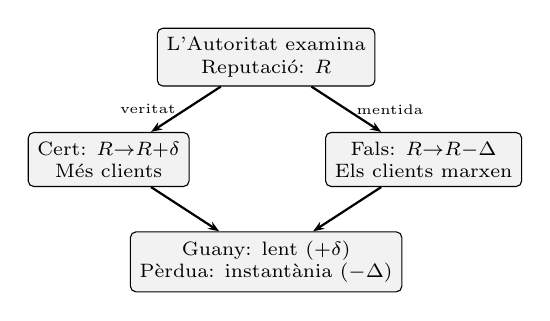
\begin{tikzpicture}[
    box/.style={draw, rounded corners=2pt, minimum width=2cm, minimum height=0.6cm, align=center, font=\scriptsize, fill=black!5},
    arr/.style={-{Stealth[length=4pt]}, thick}
]
\node[box] (exam) at (0,0) {L'Autoritat examina\\Reputació: $R$};
\node[box] (true) at (-2,-1.3) {Cert: $R{\to}R{+}\delta$\\Més clients};
\node[box] (false) at (2,-1.3) {Fals: $R{\to}R{-}\Delta$\\Els clients marxen};
\node[box] (insight) at (0,-2.6) {Guany: lent ($+\delta$)\\Pèrdua: instantània ($-\Delta$)};

\draw[arr] (exam) -- node[left,font=\tiny] {veritat} (true);
\draw[arr] (exam) -- node[right,font=\tiny] {mentida} (false);
\draw[arr] (true) -- (insight);
\draw[arr] (false) -- (insight);
\end{tikzpicture}
\caption{Autoritat de Reputació---incentius asimètrics.}
\label{fig:authority}
\end{figure}

\subsection{Reputació Multidimensional}

La reputació no és un escalar sinó un vector a través de múltiples dimensions: fiabilitat financera, integritat personal, competència professional, compromís cívic i d'altres (Fig.~\ref{fig:reputation-radar}). Els diferents proveïdors d'avaluació projecten aquest vector de manera diferent segons el context---un prestador prioritza la fiabilitat financera, un ocupador la competència professional, un veí el comportament cívic. No existeix una única puntuació de reputació ``correcta''; només perspectives.

\begin{figure}[ht]
\centering
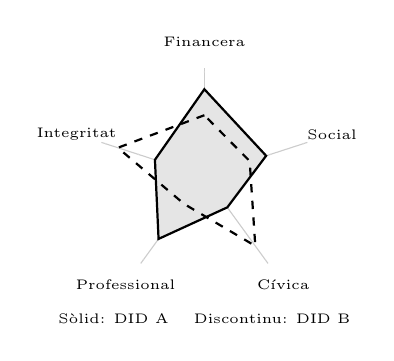
\begin{tikzpicture}[scale=0.55]
\foreach \a/\l in {90/Financera,162/Integritat,234/Professional,306/Cívica,18/Social} {
  \draw[gray!40] (0,0) -- (\a:2.5);
  \node[font=\tiny, align=center] at (\a:3.1) {\l};
  \foreach \r in {0.8,1.6,2.4} {
    \fill[black!15] (\a:\r) circle (0.5pt);
  }
}
\draw[thick, fill=black!10] (90:2.0) -- (162:1.2) -- (234:1.8) -- (306:0.9) -- (18:1.5) -- cycle;
\draw[thick, dashed] (90:1.4) -- (162:2.1) -- (234:0.8) -- (306:2.0) -- (18:1.1) -- cycle;
\node[font=\tiny] at (0,-3.3) {Sòlid: DID A \quad Discontinu: DID B};
\end{tikzpicture}
\caption{Vectors de reputació multidimensionals. Diferents DID mostren perfils diferents entre dimensions.}
\label{fig:reputation-radar}
\end{figure}

\subsection{Avaluació de Risc Democratitzada}

La RSN democratitza l'avaluació sistemàtica del risc---una capacitat actualment concentrada a les institucions financeres però aplicable molt més enllà de la banca. Els conglomerats industrials que avaluen la fiabilitat dels proveïdors, les companyies d'assegurances que posen preu al risc comportamental, la diligència deguda per a fusions i adquisicions, l'estimació de la vida útil de l'equipament a la indústria---allà on el risc de contrapart requereix avaluació, la RSN proporciona una alternativa descentralitzada i impulsada pel mercat. Un mercat de serveis d'interpretació tradueix les dades de reputació multidimensionals en brut en resums accionables, fent que l'avaluació de contrapart sigui accessible a qualsevol participant a un cost marginal.

% ============================================================
% 7. CONSENSUS AND DISPUTE RESOLUTION
% ============================================================
\section{Consens i Resolució de Disputes}

\subsection{Model de Justícia Descentralitzada}

La RSN replanteja la justícia com un problema de negociació bilateral. L'amenaça d'un dany reputacional permanent i verificable és un dissuasori més eficaç que un procediment legal que la part perjudicada no es pot permetre.

\subsection{Consens Emergent}

Cada participant manté un llindar personal de satisfacció. El consens agregat de la xarxa emergeix com la mitjana estadística de milers de negociacions bilaterals (Fig.~\ref{fig:consensus}). Una resposta molt per sobre del consens (bàrbara) és cara de publicar. Una resposta a prop del consens (proporcional) és barata. El consens no és una regla---és un senyal de preu.

\begin{figure}[ht]
\centering
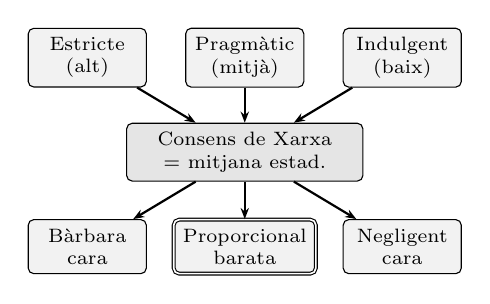
\begin{tikzpicture}[
    person/.style={draw, rounded corners=2pt, minimum width=1.5cm, minimum height=0.5cm, align=center, font=\scriptsize, fill=black!5},
    arr/.style={-{Stealth[length=4pt]}, thick}
]
\node[person] (a) at (-2,0) {Estricte\\(alt)};
\node[person] (b) at (0,0) {Pragmàtic\\(mitjà)};
\node[person] (c) at (2,0) {Indulgent\\(baix)};
\node[person, fill=black!10, minimum width=3cm] (cons) at (0,-1.2) {Consens de Xarxa\\= mitjana estad.};
\node[person] (exp) at (-2,-2.4) {Bàrbara\\cara};
\node[person, double] (prop) at (0,-2.4) {Proporcional\\barata};
\node[person] (neg) at (2,-2.4) {Negligent\\cara};

\draw[arr] (a) -- (cons);
\draw[arr] (b) -- (cons);
\draw[arr] (c) -- (cons);
\draw[arr] (cons) -- (exp);
\draw[arr] (cons) -- (prop);
\draw[arr] (cons) -- (neg);
\end{tikzpicture}
\caption{Consens emergent a partir de llindars individuals de satisfacció.}
\label{fig:consensus}
\end{figure}

\subsection{Calibratge del Càstig}

Cada Titular de DID declara públicament les respostes a categories específiques de mala conducta. Les declaracions desproporcionadament dures o indulgents atrauen senyals de reputació negatius. Les declaracions proporcionals s'accepten sense friccions---un sistema de càstig autocalibrat.

Les declaracions de consens estan elles mateixes subjectes a la detecció d'hipocresia: comprometre's declarativament amb una posició de consens mentre es comporta de manera inconsistent constitueix una infracció reputacional més greu que la desviació subjacent, ja que demostra un engany intencionat.

\subsection{Delegació}

Totes les activitats dins d'un DID---amb una excepció---es poden delegar a un altre DID. \textbf{El rol de Subjecte---el DID de qui tracta el comportament de l'afirmació---no es pot delegar; està lligat de manera intransferible al titular d'identitat a qui es refereix l'afirmació.} Els altres rols actius---Emissor, Autoritat, Testimoni, Verificador---es poden transferir a un DID delegat designat, ja sigui per a verificació, tramesa d'afirmacions, participació en el consens, o resolució de disputes. La delegació és revocable en qualsevol moment. Això possibilita l'especialització (p.\ ex., serveis professionals de verificació) mentre el Titular reté el control i la responsabilitat últims. La delegació s'aplica a tot el sistema i és essencial per a l'escalabilitat.

\subsection{De la Moralitat Individual al Contracte Social Emergent}

La política declarada de cada DID representa una formalització de la moralitat individual: què considera acceptable el Titular, com respon a comportaments específics, què exigeix de les contraparts. Aquestes polítiques no les imposa un dissenyador del sistema---les tria cada participant i s'expressen en forma llegible per màquina.

Aquesta formalització possibilita una emergència en tres etapes. Primer, la moralitat individual es codifica com a \textbf{política}---un conjunt de regles declarades, llindars i funcions de resposta que el DID es compromet a seguir. Segon, l'agregat de totes les polítiques a través de la xarxa produeix una \textbf{ètica emergent}---normes estadísticament observables que cap participant individual no va dissenyar però que sorgeixen de la interacció de milers de posicions morals individuals~\cite{durkheim1893}. Tercer, aquesta ètica emergent, expressada com a normes comportamentals compartides i fetes complir mitjançant senyals de preu bilaterals, constitueix un \textbf{contracte social mesurable}---no un constructe teòric que ningú no va signar~\cite{rawls1971}, sinó un conjunt de regles empíricament observable respatllat pel comportament real.

Aquest procés reflecteix les troballes de la teoria dels fonaments morals~\cite{haidt2012}: la moralitat humana és intuïtiva, pluralista i culturalment variable. La RSN no requereix consens moral com a entrada; produeix consens comportamental com a sortida. El contracte social resultant no és estàtic---evoluciona a mesura que els participants s'incorporen, marxen i ajusten les seves polítiques en resposta a la retroalimentació de la xarxa. A diferència de la teoria clàssica del contracte social, aquest contracte és revocable, observable i executable sense un sobirà.

% ============================================================
% 8. ECONOMIC MODEL
% ============================================================
\section{Model Econòmic}

Les seccions anteriors descrivien una eina---els mecanismes de verificació de la RSN, l'estructura de costos i el consens emergent. Aquesta secció descriu una metodologia per aplicar aquesta eina a la transició fiscal i de govern. L'eina és de propòsit general; la metodologia següent n'és una possible aplicació.

\subsection{Estructura d'Incentius}

La reputació com a capital crea incentius directes per al comportament honest. En funcionament normal, els participants construeixen reputació de manera natural mitjançant les transaccions quotidianes i els compromisos complerts. La despesa principal és en afirmacions \emph{negatives}---registrar el dany fet per altres. Aquesta asimetria incentiva un comportament útil i fiable: ser honest no costa res extra, mentre que ser perjudicial crea un rastre documentat que altres pagaran per preservar. La hipocresia---declarar regles sense seguir-les---és el mode de fallada més car, ja que demostra un engany intencionat.

\subsection{Sistema Fiscal Paral·lel}

Tres components possibiliten la pressió competitiva: (1)~\textbf{Impost Simple}---un únic tipus proporcional sense excepcions, inicialment marginalment per sota del tipus efectiu existent; (2)~\textbf{Registre Electrònic de Despesa (RED)}---invertint el model txec EET perquè els ciutadans vigilin les despeses de l'estat; (3)~\textbf{Assignació Fiscal Dirigida pel Ciutadà}---començant per un petit percentatge el primer any i arribant, després d'una dècada, a qualsevol xifra entre els percentatges de dos dígits baixos i una migració completa a un sistema dirigit pel ciutadà, segons el ritme d'adopció. El tempo real depèn de la velocitat amb què emergeixen alternatives de lliure mercat als serveis estatals i de la disposició de l'estat a cooperar amb la transició; la funció del temps no ha de ser necessàriament lineal, i no hi ha cap raó per fixar un límit superior on l'adopció pugui arribar finalment.

% ============================================================
% 9. MIGRATION PATH
% ============================================================
\section{Camí de Migració}

La migració avança a través de tres fases (Fig.~\ref{fig:migration}): \textbf{Fase~1: Superposició} (la RSN com a capa informativa, l'estat és l'únic proveïdor), \textbf{Fase~2: Competència} (la RSN proporciona alternatives funcionals, ús de doble sistema), i \textbf{Fase~3: Transició} (la RSN supera els equivalents estatals, migració voluntària). La transició és reversible en cada etapa.

\begin{figure}[ht]
\centering
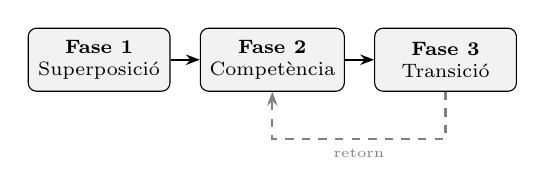
\begin{tikzpicture}[
    phase/.style={draw, rounded corners=3pt, minimum width=1.8cm, minimum height=0.8cm, align=center, font=\scriptsize, fill=black!5},
    arr/.style={-{Stealth[length=5pt]}, thick}
]
\node[phase] (p1) at (0,0) {\textbf{Fase 1}\\Superposició};
\node[phase] (p2) at (2.2,0) {\textbf{Fase 2}\\Competència};
\node[phase] (p3) at (4.4,0) {\textbf{Fase 3}\\Transició};

\draw[arr] (p1) -- (p2);
\draw[arr] (p2) -- (p3);
\draw[arr, dashed, gray] (p3.south) -- ++(0,-0.6) -| node[below,font=\tiny,pos=0.25] {retorn} (p2.south);
\end{tikzpicture}
\caption{Migració en tres fases---reversible en cada etapa.}
\label{fig:migration}
\end{figure}

El mecanisme de pressió principal és fiscal: quan els contribuents condicionals arriben a una ``minoria econòmicament significativa $X$''---un grup prou gran perquè la repressió contra ell causi un dany econòmic no trivial i la desobediència civil esdevingui una amenaça creïble---l'estat entra en negociació. A tall d'il·lustració, fem servir $X \approx 15\%$ del PIB, però el llindar real depèn de l'economia concreta.

% ============================================================
% 10. SECURITY ANALYSIS
% ============================================================
\section{Anàlisi de Seguretat}

Considerem cinc categories d'adversari: actors maliciosos individuals, grups organitzats, adversaris corporatius, adversaris a nivell d'estat i adversaris a nivell de protocol.

\textbf{Resistència Sybil}~\cite{douceur2002}. Construir reputació requereix una interacció sostinguda i verificable. El cost d'un atac Sybil reeixit escala linealment amb les identitats falses i quadràticament amb el nivell de reputació objectiu. Operar múltiples DID en paral·lel és possible però car per disseny---cada identitat ha d'acumular reputació de manera independent mitjançant una activitat genuïna. En societats lliures aquest cost dissuadeix l'abús casual; en dictadures, els DID paral·lels esdevenen una eina de supervivència que possibilita la resistència compartimentada, la coordinació clandestina i una navegació més segura pel mercat negre.

\textbf{Defensa contra la col·lusió.} Els patrons d'aval mutu entre grups tancats són detectables mitjançant l'anàlisi del graf social. Les funcions d'agregació de reputació descompten les afirmacions provinents de fonts fortament agrupades.

\textbf{Adversari a nivell d'estat.} L'encaminament onion, l'absència d'infraestructura centralitzada i la distribució del rol de Verificador entre la base de participants asseguren que la supressió requereixi mesures desproporcionades respecte de qualsevol benefici.

\textbf{Privadesa enfront de responsabilitat.} La pseudonímia---un terme mitjà entre l'anonimat i la revelació d'identitat---permet que els DID acumulin una reputació significativa sense revelar la identitat real del Titular al món.

% ============================================================
% 11. PRIVACY
% ============================================================
\section{Consideracions de Privadesa}

El model de privadesa de la RSN es construeix sobre la pseudonímia. El Titular controla la revelació d'identitat: mínima (pseudònim pur), selectiva (credencials específiques enllaçades), o completa (identitat legal associada). Les afirmacions publicades són permanents---el sistema admet la correcció contextual però no l'esborrament. Un Titular pot abandonar un DID compromès i començar de nou, renunciant a la reputació acumulada.

% ============================================================
% 12. RELATED WORK
% ============================================================
\section{Treballs Relacionats}

L'especificació W3C DID Core~\cite{did2022} i la Ceramic Network~\cite{ceramic2023} proporcionen el fonament d'identitat. EigenTrust~\cite{kamvar2003} va demostrar l'agregació distribuïda de reputació sense autoritat central. Els SBT~\cite{weyl2022} van introduir tokens socials intransferibles. La RSN es diferencia pel seu èmfasi en el cost econòmic com a filtre de qualitat i pel seu mecanisme per posar preu al radicalisme.

Les DAO~\cite{buterin2014} i la votació quadràtica~\cite{buterin2019} van demostrar la viabilitat de la governança descentralitzada. La RSN deriva el consens de negociacions bilaterals de preu en lloc de votació.

La proposta es basa en la teoria anarcocapitalista~\cite{rothbard1973,hoppe2001} per a la provisió privada de serveis però se n'aparta en dos aspectes crítics: dissenya per al ressentiment i els impulsos retributius en lloc d'assumir la racionalitat, i proposa una transició gradual en lloc de la revolució. El concepte de contractes socials emergents té antecedents en la teoria de l'ordre espontani de Hayek~\cite{hayek1973}.

\textbf{Anarcoagorisme.} La RSN comparteix un terreny comú significatiu amb la contraeconomia agorista~\cite{konkin2006}---particularment l'èmfasi a construir institucions paral·leles i l'intercanvi voluntari. Tanmateix, l'agorisme tendeix a assumir l'interès propi racional com a mecanisme de coordinació suficient i sovint manca d'un camí de migració concret des de les estructures estatals existents. La RSN incorpora explícitament tendències comportamentals no racionals i proporciona un mecanisme de pressió fiscal per a la transició gradual.

\textbf{Meritocràcia.} La RSN pot representar una primera descripció funcional de com la meritocràcia~\cite{young1958} pot emergir com a propietat sistèmica en lloc d'un eslògan. Els sistemes meritocràtics tradicionals fracassen perquè requereixen una autoritat central que defineixi i faci complir el ``mèrit''. A la RSN, el mèrit emergeix d'avaluacions bilaterals: aquells que aporten valor acumulen reputació; cap comitè no decideix qui té mèrit.

\textbf{La propietat com a privilegi.} La RSN s'aparta fonamentalment dels tractaments anarcocapitalista i de l'escola austríaca dels drets de propietat com a naturals i absoluts. En el marc de la RSN, la propietat és un \emph{privilegi}---un reconeixement social que pot, en casos extrems, ser retirat per la comunitat quan un participant viola fonamentalment les normes compartides (traïció, negativa a defensar la comunitat en una crisi existencial, explotació sistemàtica). Això no és expropiació estatal sinó una retirada del reconeixement social per part de la xarxa de relacions bilaterals.

% ============================================================
% 13. LIMITATIONS
% ============================================================
\section{Discussió i Limitacions}

\textbf{Arrencada en fred.} El valor de la RSN depèn dels efectes de xarxa; els adoptants primerencs s'enfronten a un valor limitat fins que la participació assoleix un llindar. Tanmateix, fins i tot des de les etapes inicials, la xarxa DID serveix com a font d'informació complementària útil. S'espera que l'avaluació primerenca de reputació i la valoració d'autoritats es desenvolupin gradualment amb una sofisticació creixent.

\textbf{Antiparasitisme i control d'accés.} Els DID objectiu poden imposar comissions graduades i restriccions d'accés a les consultes de DID de baixa reputació. Això no és binari sinó una escala contínua: com menys reputació té un DID consultant, menys informació rep, més espera i més paga. Aquest mecanisme incentiva la participació genuïna per sobre del consum passiu.

\textbf{Desigualtat d'accés.} El cost de publicar afirmacions pot filtrar els greuges legítims dels participants econòmicament desafavorits. Mitigació: cada participant serveix simultàniament com a verificador potencial (o delega aquest rol) i guanya comissions de verificació. En un horitzó temporal suficient, un participant no radical hauria d'acostar-se a la neutralitat financera---els ingressos per verificació compensant aproximadament els costos de publicació. Aquesta és una expectativa estadística, no una garantia.

\textbf{Desigualtat de reputació.} Els adoptants primerencs acumulen avantatges que poden crear barreres per als tardans. Tanmateix, l'avaluació de reputació la duen a terme proveïdors tercers que poden optar per mitigar l'avantatge del primer que arriba a través dels seus algorismes d'agregació. Ser el primer amb una bona reputació és un avantatge econòmic comparatiu legítim---i això és intencionat.

\textbf{Qüestions obertes.} Les funcions de cost òptimes, els estàndards d'agregació, la governança del protocol i la interacció amb dades de reputació sintètica generades per IA romanen àrees per a treball futur.

Aquest article no afirma que la RSN produeixi resultats òptims en totes les circumstàncies. Afirma que la RSN representa una alternativa \emph{factible}---tècnicament implementable, econòmicament autosostenible i socialment compatible amb les tendències comportamentals humanes tal com són realment.

% ============================================================
% 14. CONCLUSION
% ============================================================
\section{Conclusió}

Aquest article ha presentat la Xarxa Social de Reputació, un protocol descentralitzat que possibilita l'intercanvi de reputació pseudònim i verificable. El Principi del Radicalisme Costós assegura que les afirmacions fraudulentes queden excloses per preu sense censura. El camí de migració proposat possibilita una transició gradual i reversible des de les institucions existents. El disseny incorpora la naturalesa humana tal com és---incloent-hi la mesquinesa, el ressentiment i el desig de satisfacció retributiva---en lloc de requerir una transformació ideològica. El resultat no és una utopia sinó un sistema on la justícia és accessible, la reputació es guanya i el cost de la mala conducta el suporta la part que el va causar.

% ============================================================
% REFERENCES
% ============================================================
\bibliography{references}

\end{document}
